\section{Evaluation}
\label{sec:evaluation}

E1 evaluates shared workflows, E2 examines asynchronous lifecycle obligations, E3 measures scheduling interference, and E4 characterizes resource costs.

\subsection{Experimental Setup}
\label{sec:eval_setup}

Experiments used one WeAct ESP32-S3-B with one module connected at a time: a Hi-Link HLK-ZW3021 fingerprint module using the ZFM-compatible protocol, an ADH-Tech GT-511C3 fingerprint module, or a Hi-Link AI10 face/palm module. Selection covers three distinct contract mappings: staged enrollment with storage during finalization, staged enrollment with storage during the last capture, and device-managed enrollment with asynchronous completion. This diversity tests shared coordination across different acquisition and persistence boundaries. Results apply to the tested specimens and configurations.

Builds targeted \texttt{weact\_esp32s3\_b/\allowbreak{}esp32s3/\allowbreak{}procpu} using Zephyr SDK 1.0.1 and Xtensa GCC 14.3.0. Scheduling used one CPU, a reported 240~MHz cycle clock, a 10~kHz tick rate, disabled power management and time slicing, and identical fixed-work calibration across devices. UART rates were 57,600, 9,600, and 115,200 baud for ZFM-X0, GT-5X, and AI10, respectively.

One operator presented samples for functional demonstrations. Lifecycle and scheduling tests used no sample, exercising timeout and cancellation paths. Scheduling compared active workloads with initialized devices receiving no biometric calls. Resource builds used biometrics-disabled baselines with matched board and console configurations and excluded benchmark threads and trace arrays.

Applications, logs, analysis scripts, source hashes, and build records are available at \url{https://github.com/heronet/base-evaluation}. The artifact identifies the evaluated API, drivers, bindings, configurations, and software revisions; resource archives include native memory reports and object-layout records.

\subsection{E1: Shared Workflows and Functional Coverage}
\label{sec:eval_functional}

Twelve device-specific demonstrations queried capabilities, recorded the initial template-ID set, enrolled a template, checked its inventory entry, identified the same sample, exercised supported verification, and deleted the new template. All restored the initial ID set. Harnesses checked capture progress or asynchronous events and explicitly exercised unsupported operations.

A separate application used one unchanged C source for four runs, one per device/modality combination (Table~\ref{tab:eval_functional}). Build profiles supplied hardware settings and inventory limits; the shell command selected the expected modality. Capability queries selected the enrollment path and capture count without driver-name branches. Inventory comparison, identification, result checking, and removal of newly created identifiers used shared code.

\begin{table*}[t]
\centering
\caption{Functional coverage. The 12 device-specific demonstrations and four shared-application runs are separate experiments. Every shared run completed interruption, fresh enrollment, identification, and restoration of its baseline template-ID set.}
\label{tab:eval_functional}
\small
\renewcommand{\arraystretch}{1.1}
\setlength{\tabcolsep}{4pt}
\begin{tabularx}{\textwidth}{
|l|>{\raggedright\arraybackslash}X|c|c|c|}
\hline
\textbf{Device / modality} &
\textbf{Enrollment path} &
\textbf{Device-specific cycles} &
\textbf{Shared baseline = final} &
\textbf{Shared new ID} \\ \hline
ZFM-X0 / fingerprint &
Two staged captures, then finalization &
3 & $\{2\}$ & 1 \\ \hline
GT-5X / fingerprint &
Three staged captures, then finalization &
3 & $\{1\}$ & 2 \\ \hline
AI10 / face &
Device-managed; automatic identifier &
3 & $\varnothing$ & 1 \\ \hline
AI10 / palm &
Device-managed; automatic identifier &
3 & $\varnothing$ & 1001 \\ \hline
\end{tabularx}
\end{table*}

\subsubsection{Interrupted Enrollment and Reuse}
\label{sec:eval_shared_workflow}

Each shared run interrupted enrollment before performing a fresh enrollment, identification, and cleanup. Fingerprint interruption used abort after one successful capture. AI10 received no sample and was stopped after a five-second wait following acceptance. Both AI10 stops succeeded and delivered \texttt{STOPPED} with \texttt{-ECANCELED}; successful idle-only callback registration established inactivity before inventory access.

Inventory remained unchanged after interruption in all four runs. Subsequent enrollment required two captures for ZFM-X0 and three for GT-5X; AI10 delivered \texttt{ENROLL\_COMPLETE} followed by \texttt{STOPPED}(0). Identification returned the newly enrolled identifier and expected modality, and deletion restored the baseline set.

Reuse retained explicit policies: staged enrollment selected an unused identifier, managed enrollment accepted a device-assigned identifier, and termination used abort or asynchronous stop. Reconciliation required exclusive device ownership and supported inventory/deletion operations. These runs establish reuse for the exercised interruption points, not recovery after uncertain storage.

\subsubsection{Capabilities and Interface Comparison}
\label{sec:eval_interface_comparison}

Both fingerprint drivers supported identification and verification and returned \texttt{-ENOSYS} for the five tested asynchronous interfaces. AI10 rejected staged enrollment with \texttt{-ENOSYS} and synchronous verification with \texttt{-ENOTSUP}. Its six device-specific enrollments each emitted one enrollment-completion event and one terminal event.

Attribute checks confirmed rejection of unsupported settings. ZFM-X0 accepted matches at zero host threshold and rejected matches at 65,535 using separate captures; requested security level 7 was reported as 8, including after restart. GT-5X accepted valid timeout configuration and rejected invalid timeouts and unsupported threshold, enrollment-quality, and security attributes. Inventory checks used sparse databases: ZFM-X0 covered its supported first page of 100 slots, GT-5X scanned 200 configured slots, and AI10 advertised 2,000 face/palm slots.

Source inspection provides a complementary interface comparison. Adafruit Fingerprint separates feature capture, model creation, and storage~\cite{adafruit_fingerprint_library}; SparkFun GT-5X stores at its third enrollment stage~\cite{sparkfun_gt5x_family}; DFRobot AI10 exposes device-managed enrollment~\cite{dfrobot_ai10_library}. Their result conventions differ, while GROW R502A uses private sensor attributes and biometric interpretations of \texttt{sensor\_value}~\cite{zephyr_r502a}. BASE places these differences behind common operations and typed results while retaining capability-dependent workflows.

The inspected Arduino interfaces do not expose a public terminal-callback and callback-quiescence contract; GROW's touch trigger indicates sample presence rather than operation completion. This comparison identifies semantic differences, not measured performance advantages over those implementations.

\subsection{E2: Lifecycle and Callback Quiescence}
\label{sec:eval_lifecycle}

AI10 tests exercised the obligations in Section~\ref{sec:correctness_properties}. The first suite covered enrollment timeout, single-attempt identification timeout, enrollment and continuous-identification cancellation with zero or 1,000~ms added delay, and conflicting requests during continuous identification. Each case was followed by a start/stop recovery probe. Three repetitions yielded 21 primary and 21 recovery operations, tracked using instrumentation-local identifiers rather than API tokens.

All 42 operations emitted exactly one \texttt{STOPPED}, without reported event-buffer loss. Enrollment timeout produced \texttt{ERROR} and \texttt{STOPPED}, both with \texttt{-ETIMEDOUT}; identification timeout produced \texttt{NO\_MATCH} with timeout status followed by \texttt{STOPPED}(0). The other 36 operations terminated with cancellation status. Callback-context checks passed, conflicts were rejected, recovery completed, and inventory remained unchanged.

Successful stop calls took 14--55~ms, including recovery and busy-operation cases; Figure~\ref{fig:eval_lifecycle}(a) shows the primary cancellation cases. Measurements used millisecond uptime around the helper's invocation and include scheduling and coordination overhead; they are observations, not bounds.

\begin{figure*}[t]
\centering
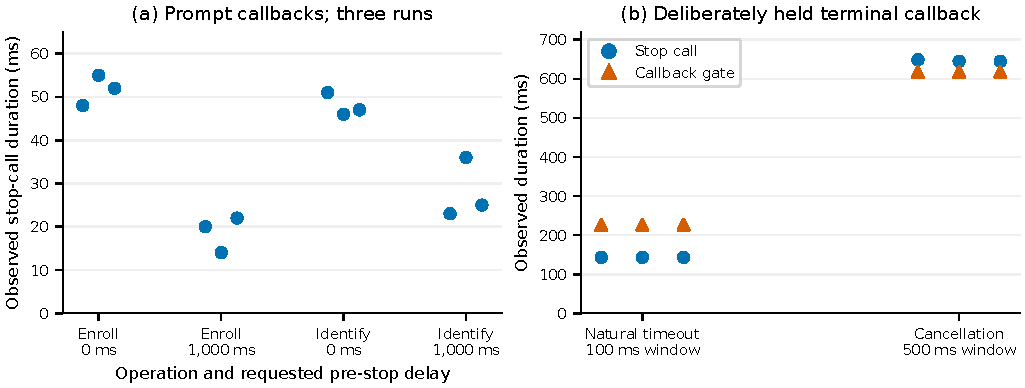
\includegraphics[width=\textwidth]{figures/fig_eval_lifecycle.pdf}
\caption{AI10 stop behavior. (a) Three observations per primary cancellation case with promptly returning callbacks; zero delay means no added sleep before stop. (b) Separate held-callback tests with 100 or 500~ms added observation windows. Gate duration includes probes and logging; these stress timings must not be pooled with ordinary cancellation latency.}
\label{fig:eval_lifecycle}
\end{figure*}

A second suite held the terminal callback on a semaphore during natural enrollment timeout and continuous-identification cancellation. Three repetitions per case produced six held callbacks and six subsequent recovery operations. All 24 enrollment, identification, callback-replacement, and inventory probes returned \texttt{-EBUSY}. Natural-timeout probes preceded the first stop call, excluding a stopping caller's mutex as the sole explanation. A second stop caller was rejected in all six cases.

The primary stop remained pending through the added observation window. After gate release, the marker immediately before callback return preceded the marker after stop return, and recovery succeeded. Natural-timeout stop calls took 143~ms; cancellation stop calls took 645--649~ms (Figure~\ref{fig:eval_lifecycle}(b)). The exact callback-return instruction was not instrumented, and millisecond timestamp equality does not imply zero delay.

Across both suites, all 54 accepted operations produced one terminal event. The observed exclusion, pending-stop behavior, and marker ordering support the specified obligations for the tested schedules and demonstrate the effect of callback duration on availability.

\subsection{E3: Scheduling Responsiveness}
\label{sec:eval_scheduling}

A periodic task performed fixed integer work calibrated to approximately 200~$\mu$s, with a 10~ms period and relative deadline. Its priority was 2 or 8; lower values take precedence. Biometric work used priority~5. Optional background work at priority~4 executed a calibrated 3,513~$\mu$s every 7~ms, representing 50.19\% offered computation rather than measured CPU utilization.

Each device ran initialized-idle and repeated synchronous identification conditions, the latter with a separate caller and one-second timeout. AI10 additionally ran asynchronous single-attempt identification, waiting for termination and callback quiescence before restarting; its coordinator and worker both used priority~5. Synchronous callers suspended normally without scheduler locking or artificial busy-waiting.

After a 200~ms settling interval, each condition recorded 300 periodic jobs over approximately three seconds. Active conditions required a completed biometric cycle within the window; in-flight work was drained afterward. Records were buffered and printed after measurement.

For timer-callback release $r_i$, task start $s_i$, finish $f_i$, and cycle frequency $f_c$, the recorded quantities were
\begin{equation}
D_i=\frac{s_i-r_i}{f_c},\quad
R_i=\frac{f_i-r_i}{f_c},\quad
W_i=\frac{f_i-s_i}{f_c}.
\label{eq:eval_timing}
\end{equation}
Here $D_i$ is release-to-start latency, $R_i$ response time, and $W_i$ execution span including preemption. A miss means $R_i>10$~ms. This definition excludes lateness before the timer-callback timestamp and does not measure response against an ideal external schedule.

Three suites per device, with 12 AI10 or eight fingerprint conditions per suite, produced 25,200 jobs across 84 measurement cells. Suites are repetitions; jobs within a suite are correlated observations. Mode order varied, while device and priority/load group orders remained fixed. Checks covered receive status, job counts, queue loss, timestamp ordering and wrap, and workload progress. Percentiles use linear interpolation within each 300-job cell, retaining the three suite results separately.

\begin{figure*}[t]
\centering
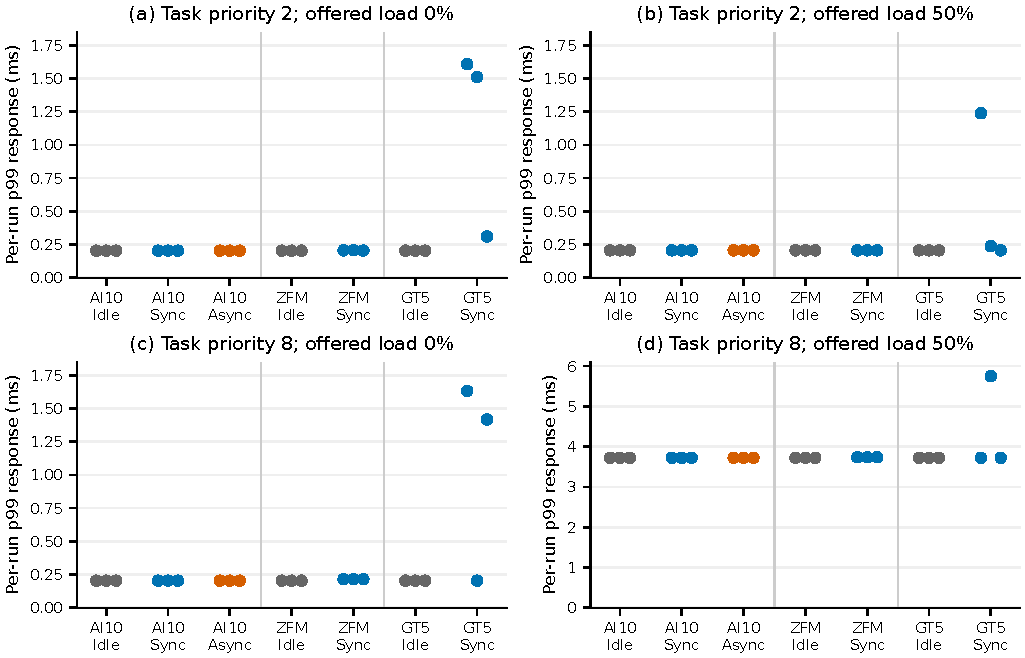
\includegraphics[width=\textwidth]{figures/fig_eval_p99.pdf}
\caption{Per-run 99th-percentile response times: 84 points, each summarizing 300 jobs, with three points per condition. Priority~2 places the task above the workload threads; priority~8 places it below them. Panel~(d) uses a different vertical scale. Asynchronous operation is tested only on AI10.}
\label{fig:eval_p99}
\end{figure*}

All suites passed completeness and progress checks without queue loss, receive errors, or observed deadline misses. Figure~\ref{fig:eval_p99} summarizes per-run 99th-percentile response times. AI10's priority-2 maxima did not exceed 0.213~ms. ZFM-X0 synchronous maxima approached 0.641~ms despite 99th percentiles near idle. GT-5X showed greater variation: its unloaded priority-2 synchronous 99th percentiles were 1.608, 1.511, and 0.311~ms (Figure~\ref{fig:eval_p99}).

At priority~8 with background load, idle maxima were approximately 3.722~ms. Active maxima were 3.764/3.765~ms for synchronous/asynchronous AI10, 4.163~ms for ZFM-X0, and 6.333~ms for GT-5X. GT-5X's loaded synchronous 99th percentiles ranged from approximately 3.722 to 5.747~ms. Figure~\ref{fig:eval_ecdf} retains individual-run distributions rather than pooling their differing tails.

\begin{figure*}[!h]
\centering
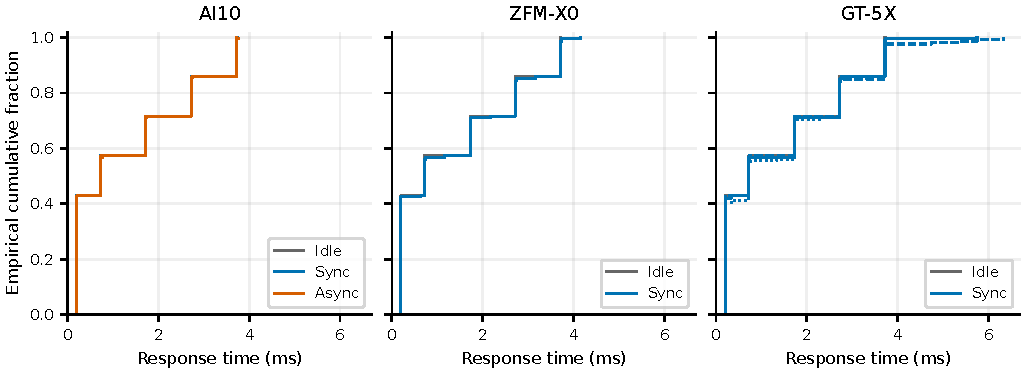
\includegraphics[width=\textwidth]{figures/fig_eval_ecdf.pdf}
\caption{Response-time distributions at priority~8 with nominal 50\% offered background computation. Each curve contains 300 jobs; the subset contains 21 curves and 6,300 jobs. Line styles distinguish the three runs. Curves may overlap.}
\label{fig:eval_ecdf}
\end{figure*}

The measurements capture combined effects of UART rates, traffic, synchronization, and module responses; they do not isolate the cause of GT-5X's spikes. AI10's synchronous and asynchronous interference was similar under the no-sample workload, consistent with synchronous callers suspending while unrelated work proceeds. Observed maxima are not worst-case bounds.

\subsection{E4: Resource Footprint}
\label{sec:eval_resources}

Each driver had biometrics-disabled UART/console, initialized-idle, and synchronous-identification builds; AI10 also had an asynchronous build. All used size optimization, a 4,096-byte main stack, disabled shell/logging, and no stack-fill profiling. Separate instrumented builds enabled stack initialization and an observer.

Table~\ref{tab:eval_memory} reports increments from Zephyr's native linked ROM/RAM reports. Every matched baseline contained 57,600 bytes ROM and 126,204 bytes RAM. Increments include application code, dependencies, and alignment; ESP32 executable RAM and shared platform storage require linker-map interpretation.

\begin{table}[t]
\centering
\caption{Linked-image increments over matched baselines, in bytes. Instrumented stack-profile builds are excluded.}
\label{tab:eval_memory}
\small
\renewcommand{\arraystretch}{1.1}
\setlength{\tabcolsep}{5pt}
\begin{tabular}{|l|l|r|r|}
\hline
\textbf{Driver} & \textbf{Mode} &
$\Delta$\textbf{ROM} & $\Delta$\textbf{RAM} \\ \hline
ZFM-X0 & Idle  & 4,924 & 648 \\ \hline
ZFM-X0 & Sync  & 4,972 & 648 \\ \hline
GT-5X  & Idle  & 5,172 & 152 \\ \hline
GT-5X  & Sync  & 5,220 & 152 \\ \hline
AI10   & Idle  & 5,280 & 3,824 \\ \hline
AI10   & Sync  & 5,328 & 3,824 \\ \hline
AI10   & Async & 5,712 & 3,840 \\ \hline
\end{tabular}
\end{table}

Synchronous integration added 4,972--5,328 bytes ROM. AI10 reserves its 2,048-byte worker stack, 1,024-byte receive ring, packet storage, and synchronization state even in idle and synchronous builds. Its asynchronous application therefore adds only 384 bytes ROM and 16 bytes RAM over the synchronous image.

GT-5X's 152-byte instance contains a pointer to heap storage. Source inspection identifies simultaneous initialization requests for a persistent 498-byte template buffer and a temporary 30-byte packet: 528 payload bytes, excluding allocator overhead and fragmentation. Template transfers would request another 504-byte packet but were not profiled. These are requested sizes, not measured peak heap use. Heap backing storage is already included in linked RAM; adding these payloads to image totals would double-count it, while the instance size alone omits runtime demand.

At quiescent checkpoints, an observer scanned the blocked application stack and AI10 worker. Each device completed three no-sample synchronous attempts; AI10 additionally completed three asynchronous timeouts and three continuous-recognition cancellations. Maximum observed main-stack watermarks were 576, 592, and 688 bytes for ZFM-X0, GT-5X, and AI10, respectively, from 4,096-byte stacks. AI10's worker watermark was 528 bytes from 2,048 bytes.

Watermarks include startup and harness work, and the worker measurement includes the test callback. They characterize the exercised workloads, not worst-case stack requirements; an unchanged watermark does not imply zero stack use.

\subsection{Research Question Answers and Limitations}
\label{sec:eval_limits}

For RQ1, one application source reused coordination across three device families through capability-dependent workflows while retaining explicit allocation, termination, and recovery policies. For RQ2, all 54 accepted operations delivered one terminal event, and directed checks supported exclusion and callback quiescence for the tested schedules. For RQ3, interference varied with driver, priority, and load; AI10's synchronous and asynchronous paths behaved similarly under the no-sample workload. For RQ4, linked-image costs and observed stack usage exposed implementation-dependent allocation choices, including worker storage retained during synchronous use. Together, these findings support reusable coordination while requiring configuration-specific timing and memory assessment.

Coverage is limited to one board, one specimen per family, and one operator. Functional runs establish workflow behavior, not recognition accuracy or calibrated security equivalence. Shared recovery tests cover staged abort after one capture and AI10 cancellation without a sample; they do not establish recovery after uncertain storage.

Asynchronous lifecycle evidence is limited to AI10 and the directed schedules. Delayed stops across ownership handoff, completion/cancellation races, cleanup failure after acknowledged storage, and systematic UART fault injection were not evaluated. Scheduling evidence covers short, no-sample workloads with three suites per device and fixed device and priority/load group orders.
